\subsection{Overview}

Goal of this study is to asses the stability of fit in the 2D analysis in terms of yield normalization for the main processes.
We look at the fit output normalization and compare it with the input value to the card, both for the background only fit and for the signal+background fit.
The \mHi=125 \GeV\ analysis is taken as reference and is studied in three cases: no injection, \mHi\=125 \GeV\ injected, \mHi\=200 \GeV injected.
Input shapes and normalizations are nominal, i.e. we are not testing the e􏰁ect of systematic variation but only of statistical;
toys are performed based on poisson sampling and backgrounds are not re-evaluated for each toy.

%%%%%%%%%%%% NO INJECTION %%%%%%%%%%%%
\subsection{Analysis with no injected signal}

Post-fit normalization results are summarized in Figures~\ref{fig:norm_injdef_0j_125_bfit}-\ref{fig:norm_injdef_1j_125_sfit}.
No significant biases are observed; background only and signal+background fits agree.
Best constrained processes are qqWW in 0-jet bin ($\sigma$~3\%) and Top in 1-jet bin Top ($\sigma$~4\%); 
worst constrained processes are Wgamma ($\sigma$~40\%) and Wjets ($\sigma$~20\%).

%%%%%%%%%%%%%%%%%%%%
\begin{figure}[!hbtp]
\centering
\subfigure[qqWW]{
\centering
\label{subfig:norm_injdef_0j_125_bfit_qqWW}
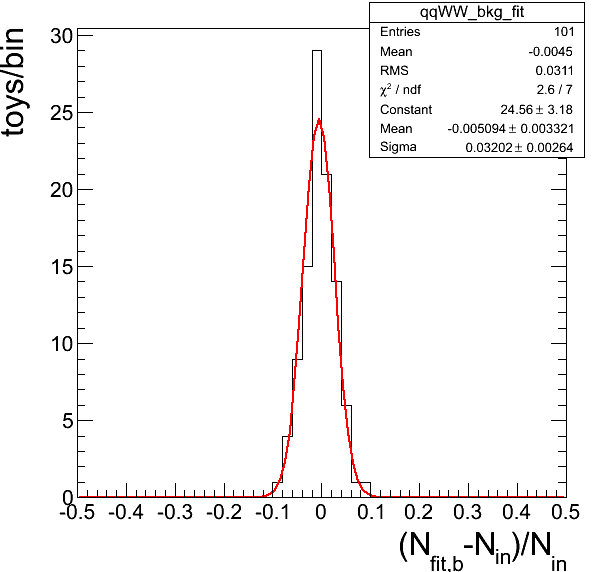
\includegraphics[width=.38\textwidth]{figures/norm_injdef_0j_125_bfit_qqWW.png}
}
\subfigure[ggWW]{
\centering
\label{subfig:norm_injdef_0j_125_bfit_ggWW}
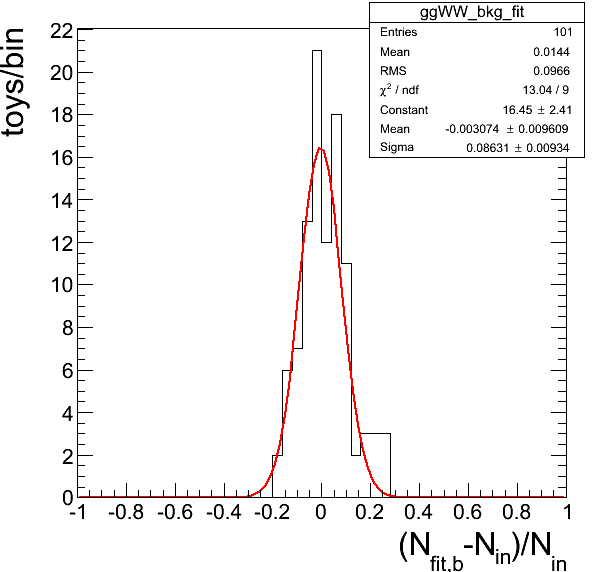
\includegraphics[width=.38\textwidth]{figures/norm_injdef_0j_125_bfit_ggWW.png}
}
\\
\subfigure[Wjets]{
\centering
\label{subfig:norm_injdef_0j_125_bfit_Wjets}
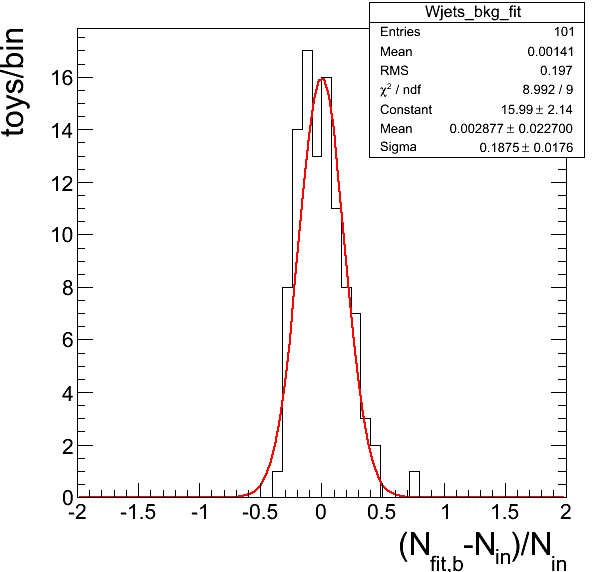
\includegraphics[width=.38\textwidth]{figures/norm_injdef_0j_125_bfit_Wjets.png}
}
\subfigure[Wgamma]{
\centering
\label{subfig:norm_injdef_0j_125_bfit_Wgamma}
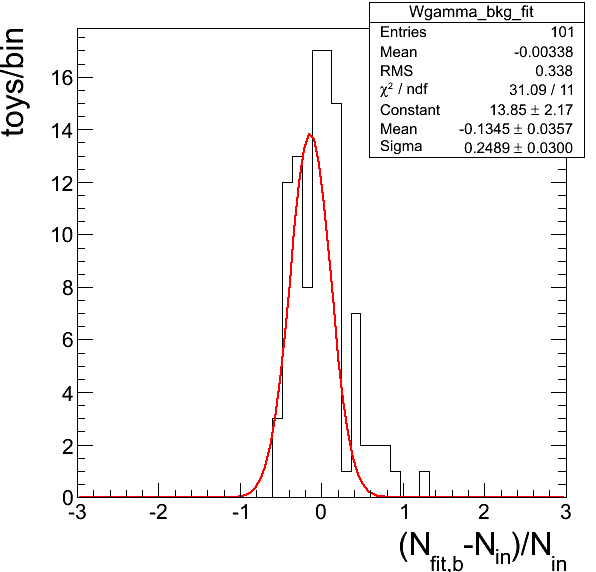
\includegraphics[width=.38\textwidth]{figures/norm_injdef_0j_125_bfit_Wgamma.png}
}
\\
\subfigure[Top]{
\centering
\label{subfig:norm_injdef_0j_125_bfit_Top}
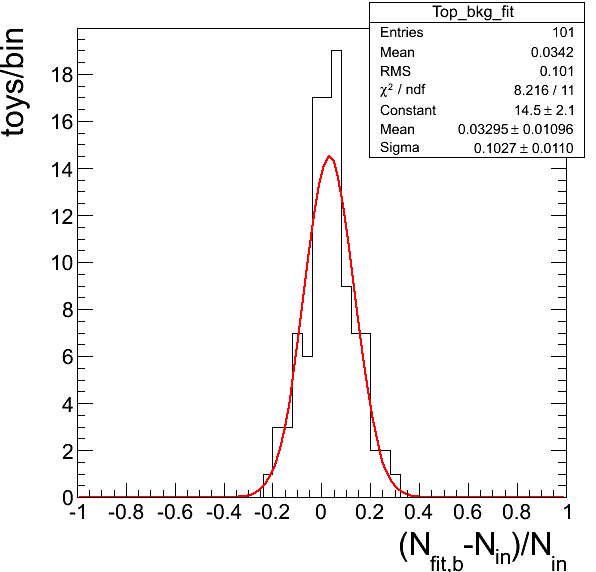
\includegraphics[width=.38\textwidth]{figures/norm_injdef_0j_125_bfit_Top.png}
}
\subfigure[ggH]{
\centering
\label{subfig:norm_injdef_0j_125_bfit_ggH}
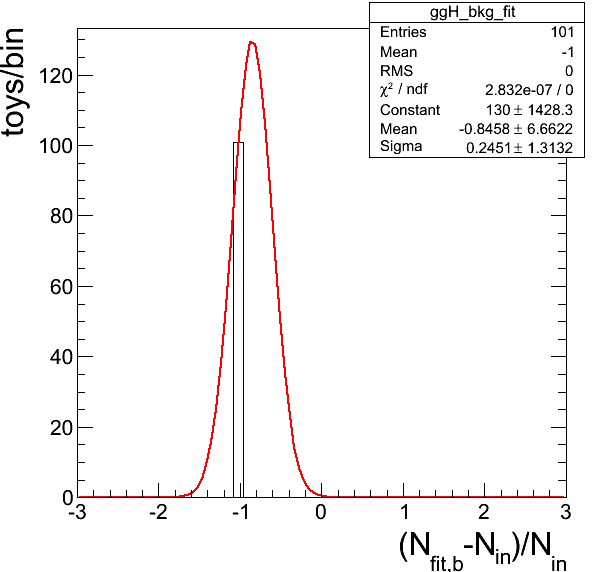
\includegraphics[width=.38\textwidth]{figures/norm_injdef_0j_125_bfit_ggH.png}
}
\caption{Relative shift of post-fit normalization for \mHi=125 \GeV, 0-jet 2D analysis.
No signal injection. Results of background only fit are shown.}
\label{fig:norm_injdef_0j_125_bfit}
\end{figure}
%%%%%%%%%%%%%%%%%%%%

%%%%%%%%%%%%%%%%%%%%
\begin{figure}[!hbtp]
\centering
\subfigure[qqWW]{
\centering
\label{subfig:norm_injdef_0j_125_sfit_qqWW}
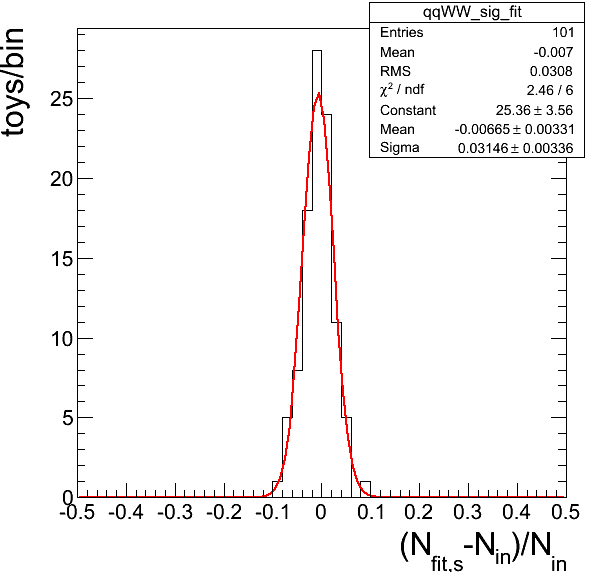
\includegraphics[width=.38\textwidth]{figures/norm_injdef_0j_125_sfit_qqWW.png}
}
\subfigure[ggWW]{
\centering
\label{subfig:norm_injdef_0j_125_sfit_ggWW}
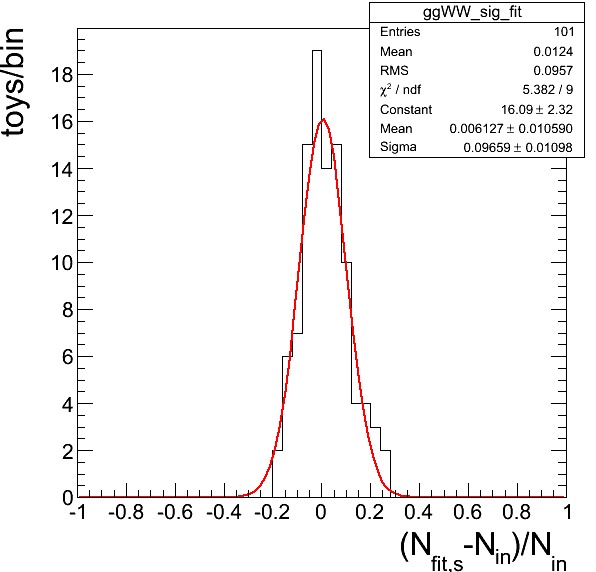
\includegraphics[width=.38\textwidth]{figures/norm_injdef_0j_125_sfit_ggWW.png}
}
\\
\subfigure[Wjets]{
\centering
\label{subfig:norm_injdef_0j_125_sfit_Wjets}
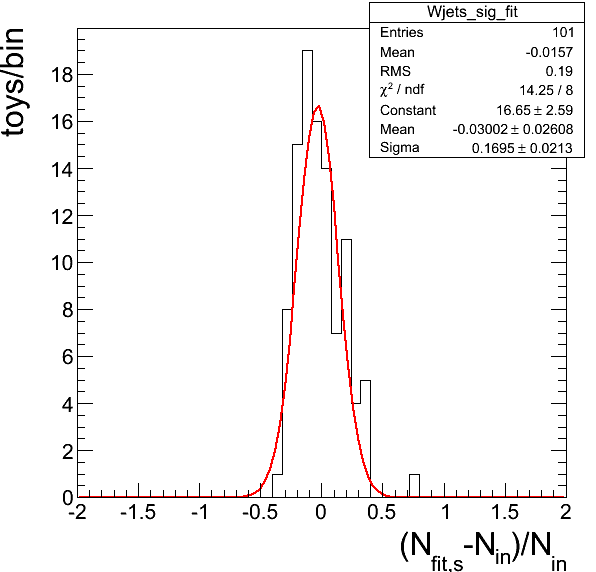
\includegraphics[width=.38\textwidth]{figures/norm_injdef_0j_125_sfit_Wjets.png}
}
\subfigure[Wgamma]{
\centering
\label{subfig:norm_injdef_0j_125_sfit_Wgamma}
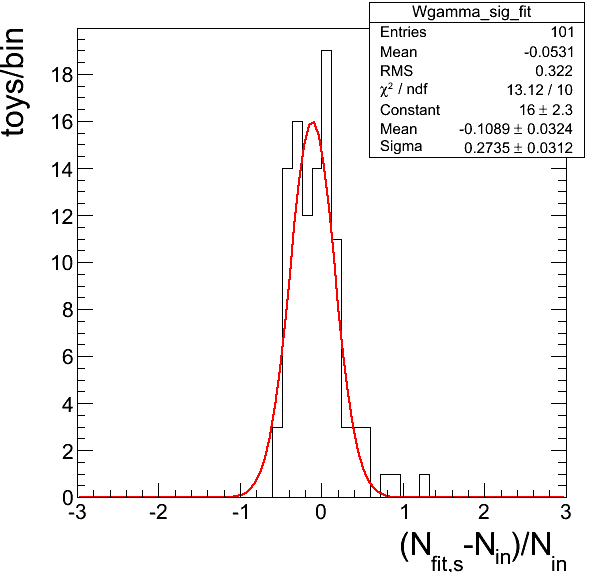
\includegraphics[width=.38\textwidth]{figures/norm_injdef_0j_125_sfit_Wgamma.png}
}
\\
\subfigure[Top]{
\centering
\label{subfig:norm_injdef_0j_125_sfit_Top}
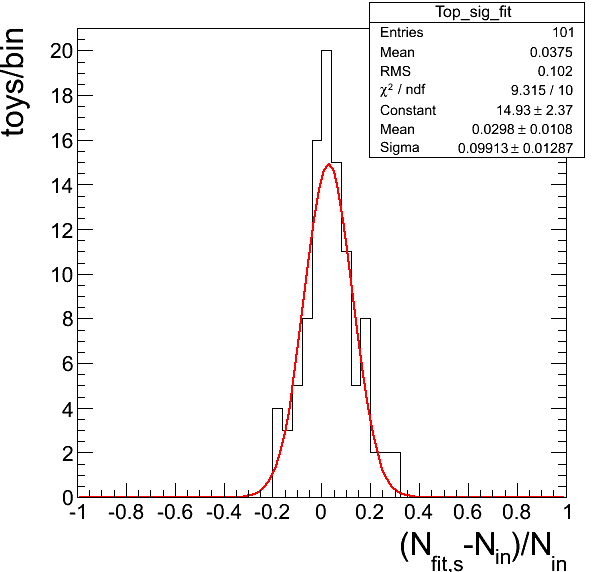
\includegraphics[width=.38\textwidth]{figures/norm_injdef_0j_125_sfit_Top.png}
}
\subfigure[ggH]{
\centering
\label{subfig:norm_injdef_0j_125_sfit_ggH}
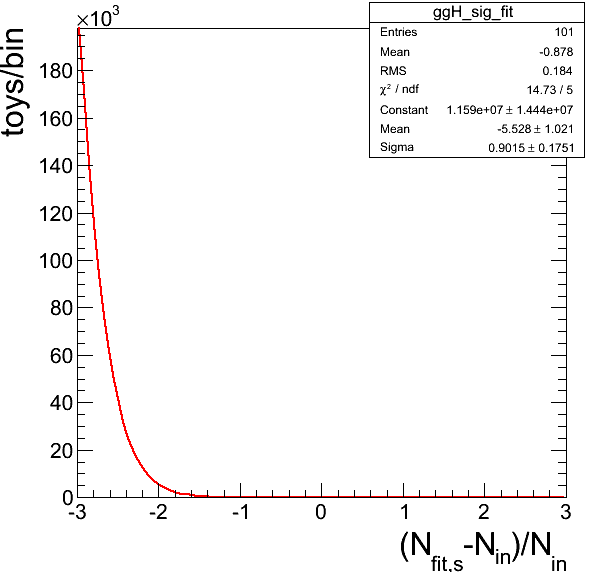
\includegraphics[width=.38\textwidth]{figures/norm_injdef_0j_125_sfit_ggH.png}
}
\caption{Relative shift of post-fit normalization for \mHi=125 \GeV, 0-jet 2D analysis.
No signal injection. Results of background+signal fit are shown.}
\label{fig:norm_injdef_0j_125_sfit}
\end{figure}
%%%%%%%%%%%%%%%%%%%%

%%%%%%%%%%%%%%%%%%%%
\begin{figure}[!hbtp]
\centering
\subfigure[qqWW]{
\centering
\label{subfig:norm_injdef_1j_125_bfit_qqWW}
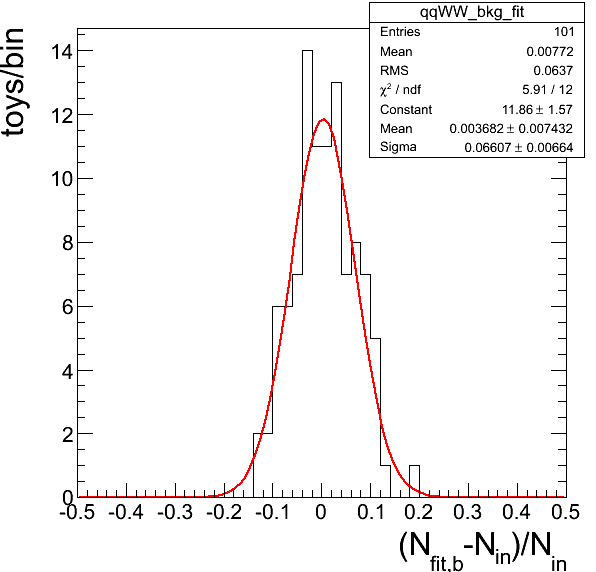
\includegraphics[width=.38\textwidth]{figures/norm_injdef_1j_125_bfit_qqWW.png}
}
\subfigure[ggWW]{
\centering
\label{subfig:norm_injdef_1j_125_bfit_ggWW}
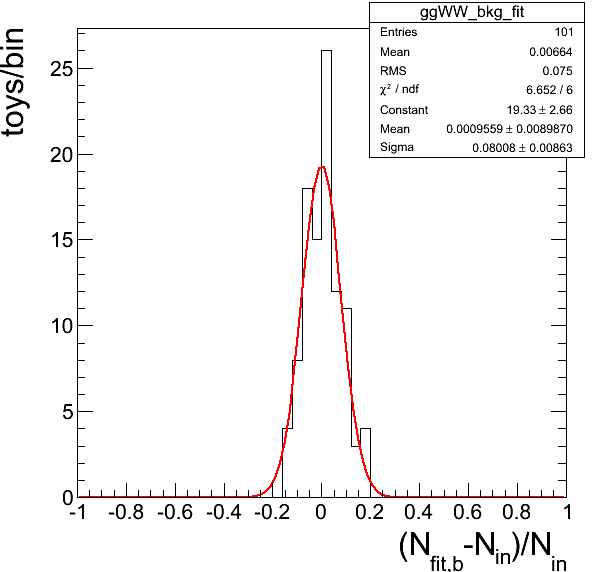
\includegraphics[width=.38\textwidth]{figures/norm_injdef_1j_125_bfit_ggWW.png}
}
\\
\subfigure[Wjets]{
\centering
\label{subfig:norm_injdef_1j_125_bfit_Wjets}
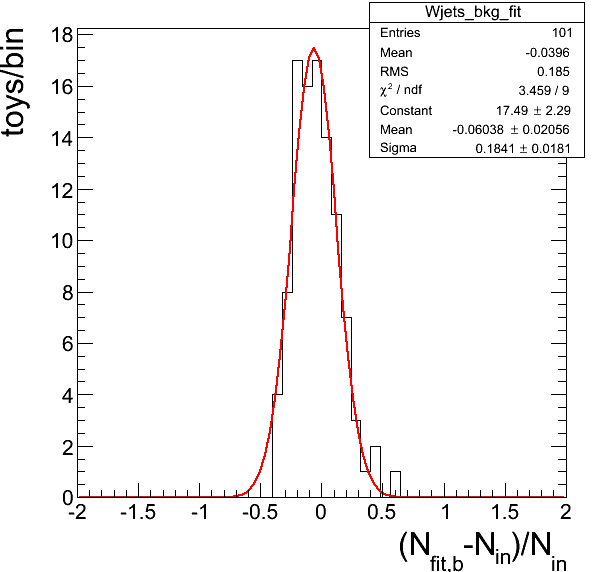
\includegraphics[width=.38\textwidth]{figures/norm_injdef_1j_125_bfit_Wjets.png}
}
\subfigure[Wgamma]{
\centering
\label{subfig:norm_injdef_1j_125_bfit_Wgamma}
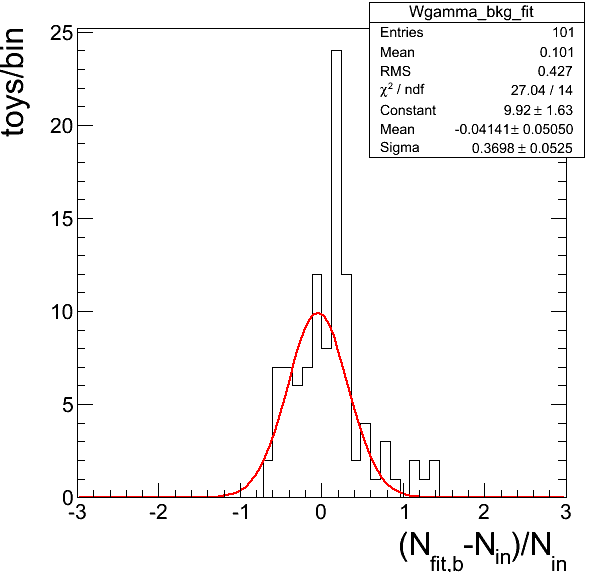
\includegraphics[width=.38\textwidth]{figures/norm_injdef_1j_125_bfit_Wgamma.png}
}
\\
\subfigure[Top]{
\centering
\label{subfig:norm_injdef_1j_125_bfit_Top}
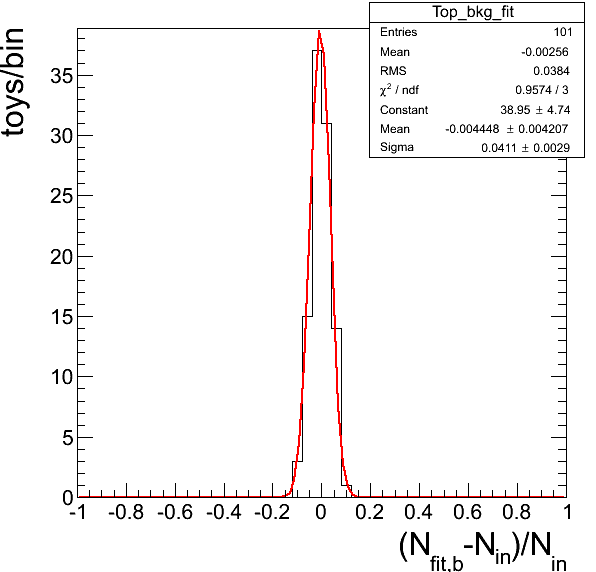
\includegraphics[width=.38\textwidth]{figures/norm_injdef_1j_125_bfit_Top.png}
}
\subfigure[ggH]{
\centering
\label{subfig:norm_injdef_1j_125_bfit_ggH}
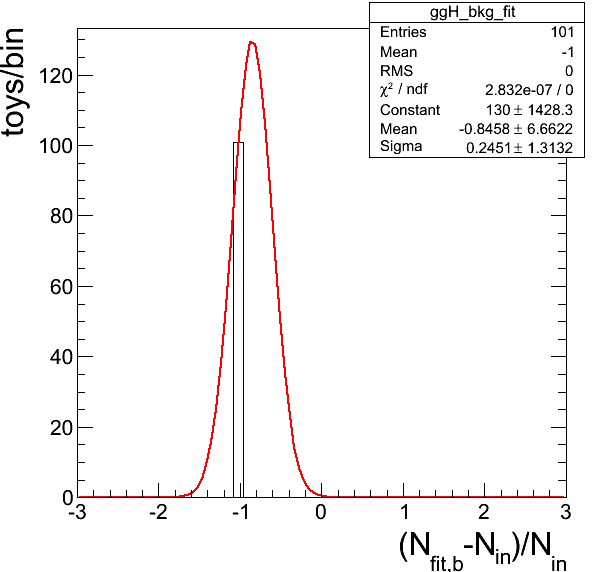
\includegraphics[width=.38\textwidth]{figures/norm_injdef_1j_125_bfit_ggH.png}
}
\caption{Relative shift of post-fit normalization for \mHi=125 \GeV, 1-jet 2D analysis.
No signal injection. Results of background only fit are shown.}
\label{fig:norm_injdef_1j_125_bfit}
\end{figure}
%%%%%%%%%%%%%%%%%%%%

%%%%%%%%%%%%%%%%%%%%
\begin{figure}[!hbtp]
\centering
\subfigure[qqWW]{
\centering
\label{subfig:norm_injdef_1j_125_sfit_qqWW}
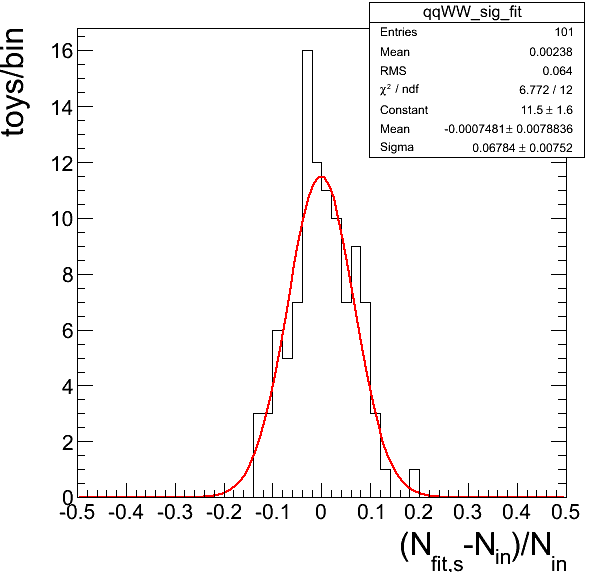
\includegraphics[width=.38\textwidth]{figures/norm_injdef_1j_125_sfit_qqWW.png}
}
\subfigure[ggWW]{
\centering
\label{subfig:norm_injdef_1j_125_sfit_ggWW}
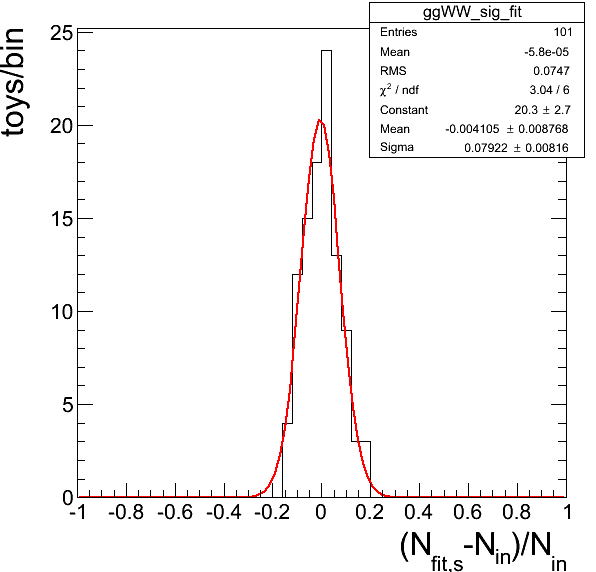
\includegraphics[width=.38\textwidth]{figures/norm_injdef_1j_125_sfit_ggWW.png}
}
\\
\subfigure[Wjets]{
\centering
\label{subfig:norm_injdef_1j_125_sfit_Wjets}
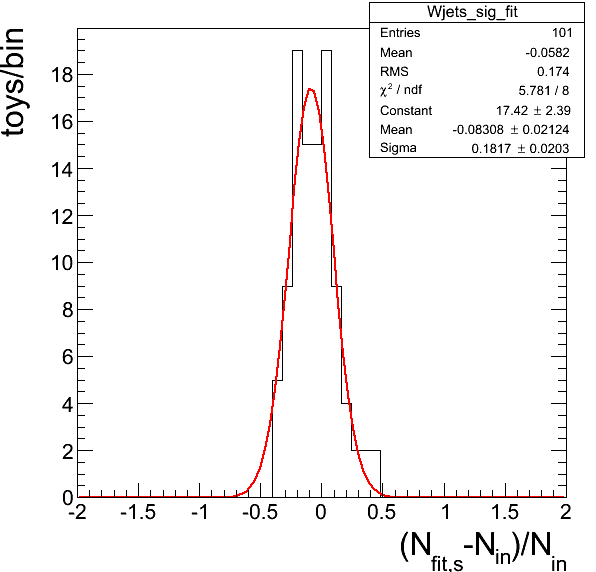
\includegraphics[width=.38\textwidth]{figures/norm_injdef_1j_125_sfit_Wjets.png}
}
\subfigure[Wgamma]{
\centering
\label{subfig:norm_injdef_1j_125_sfit_Wgamma}
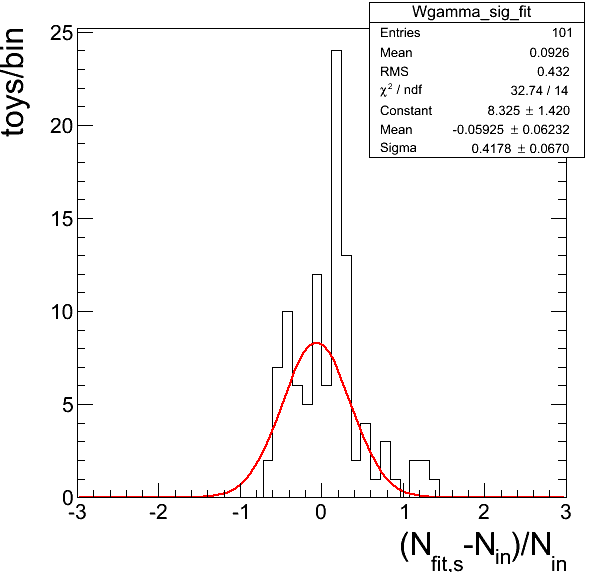
\includegraphics[width=.38\textwidth]{figures/norm_injdef_1j_125_sfit_Wgamma.png}
}
\\
\subfigure[Top]{
\centering
\label{subfig:norm_injdef_1j_125_sfit_Top}
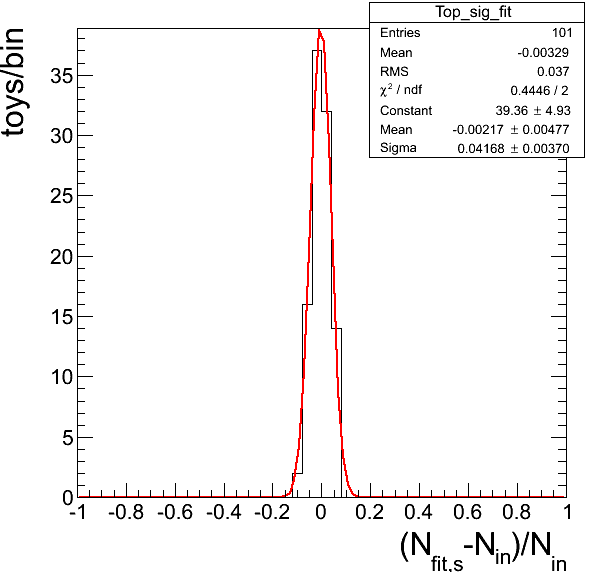
\includegraphics[width=.38\textwidth]{figures/norm_injdef_1j_125_sfit_Top.png}
}
\subfigure[ggH]{
\centering
\label{subfig:norm_injdef_1j_125_sfit_ggH}
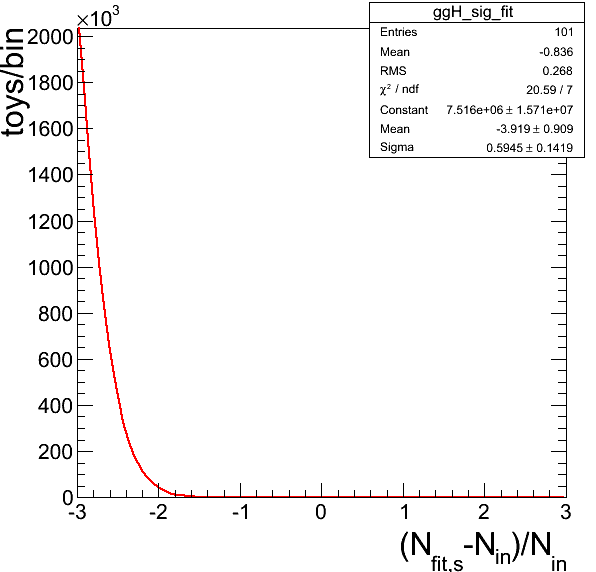
\includegraphics[width=.38\textwidth]{figures/norm_injdef_1j_125_sfit_ggH.png}
}
\caption{Relative shift of post-fit normalization for \mHi=125 \GeV, 1-jet 2D analysis.
No signal injection. Results of background+signal fit are shown.}
\label{fig:norm_injdef_1j_125_sfit}
\end{figure}
%%%%%%%%%%%%%%%%%%%%

\clearpage

%%%%%%%%%%%% MH=125 INJECTION %%%%%%%%%%%%
\subsection{Analysis with \mHi=125 \GeV\ SM Higgs injected}

Post-fit normalization results are summarized in Figures~\ref{fig:norm_inj125_0j_125_bfit}-\ref{fig:norm_inj125_1j_125_sfit}.
Signal is absorbed by backgrounds in background-only fit: Wgamma and Wjets are biassed by ~35\% and ~20\% respectively.
Signal fit shows no biases and the Higgs yield is measured with $\sigma$~40\% (60\%) in 0-jet (1-jet) bin.

%%%%%%%%%%%%%%%%%%%%
\begin{figure}[!hbtp]
\centering
\subfigure[qqWW]{
\centering
\label{subfig:norm_inj125_0j_125_bfit_qqWW}
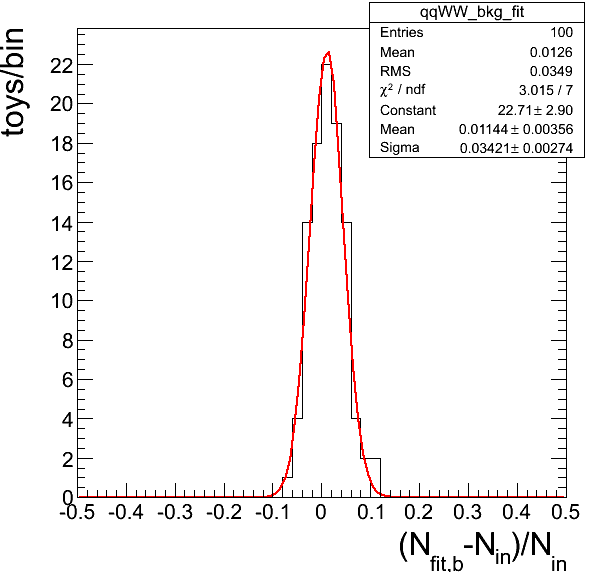
\includegraphics[width=.38\textwidth]{figures/norm_inj125_0j_125_bfit_qqWW.png}
}
\subfigure[ggWW]{
\centering
\label{subfig:norm_inj125_0j_125_bfit_ggWW}
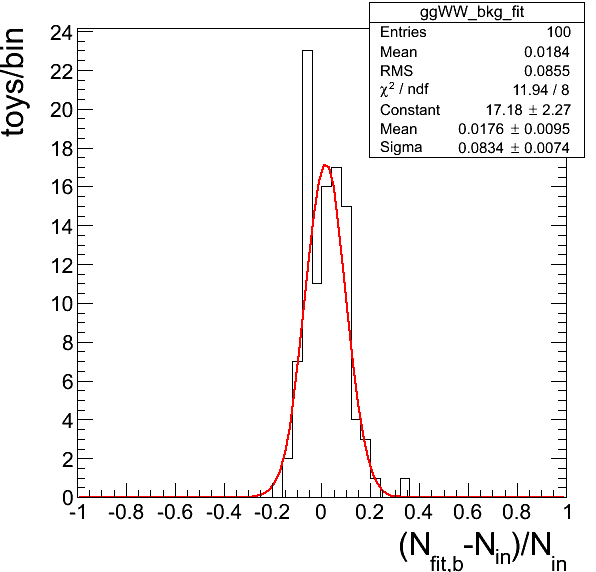
\includegraphics[width=.38\textwidth]{figures/norm_inj125_0j_125_bfit_ggWW.png}
}
\\
\subfigure[Wjets]{
\centering
\label{subfig:norm_inj125_0j_125_bfit_Wjets}
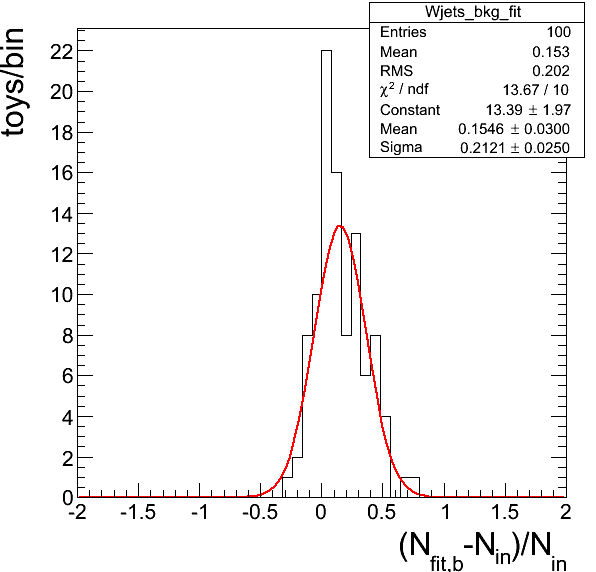
\includegraphics[width=.38\textwidth]{figures/norm_inj125_0j_125_bfit_Wjets.png}
}
\subfigure[Wgamma]{
\centering
\label{subfig:norm_inj125_0j_125_bfit_Wgamma}
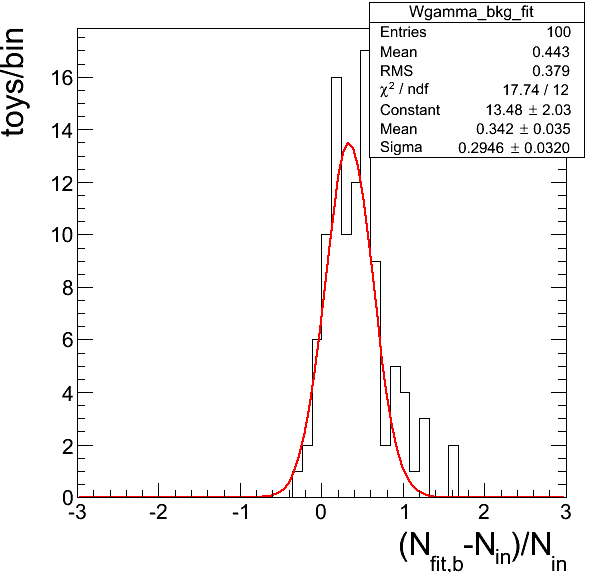
\includegraphics[width=.38\textwidth]{figures/norm_inj125_0j_125_bfit_Wgamma.png}
}
\\
\subfigure[Top]{
\centering
\label{subfig:norm_inj125_0j_125_bfit_Top}
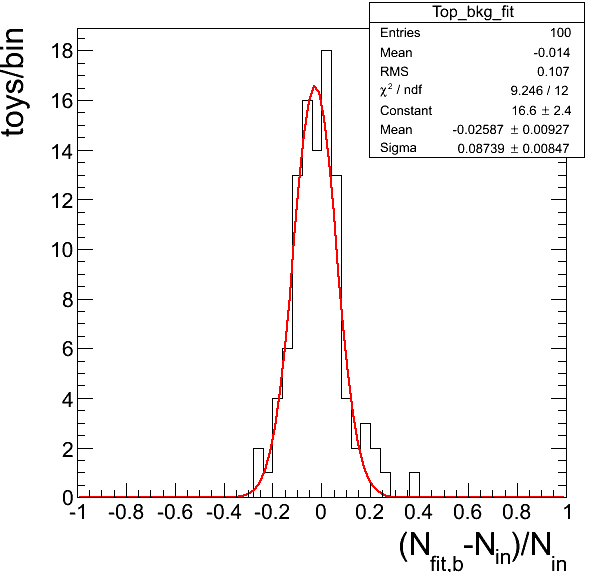
\includegraphics[width=.38\textwidth]{figures/norm_inj125_0j_125_bfit_Top.png}
}
\subfigure[ggH]{
\centering
\label{subfig:norm_inj125_0j_125_bfit_ggH}
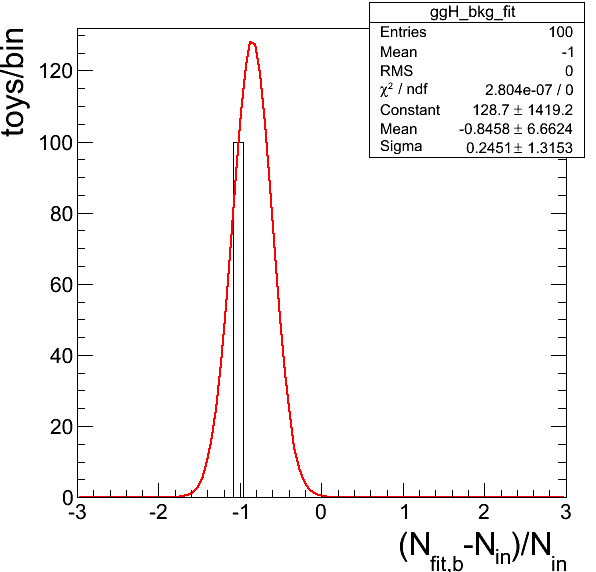
\includegraphics[width=.38\textwidth]{figures/norm_inj125_0j_125_bfit_ggH.png}
}
\caption{Relative shift of post-fit normalization for \mHi=125 \GeV, 0-jet 2D analysis.
A SM Higgs signal with \mHi=125 \GeV\ is injected. Results of background only fit are shown.}
\label{fig:norm_inj125_0j_125_bfit}
\end{figure}
%%%%%%%%%%%%%%%%%%%%

%%%%%%%%%%%%%%%%%%%%
\begin{figure}[!hbtp]
\centering
\subfigure[qqWW]{
\centering
\label{subfig:norm_inj125_0j_125_sfit_qqWW}
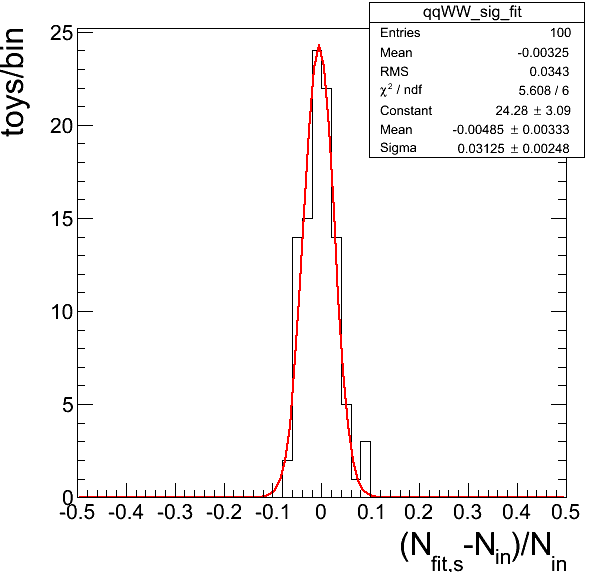
\includegraphics[width=.38\textwidth]{figures/norm_inj125_0j_125_sfit_qqWW.png}
}
\subfigure[ggWW]{
\centering
\label{subfig:norm_inj125_0j_125_sfit_ggWW}
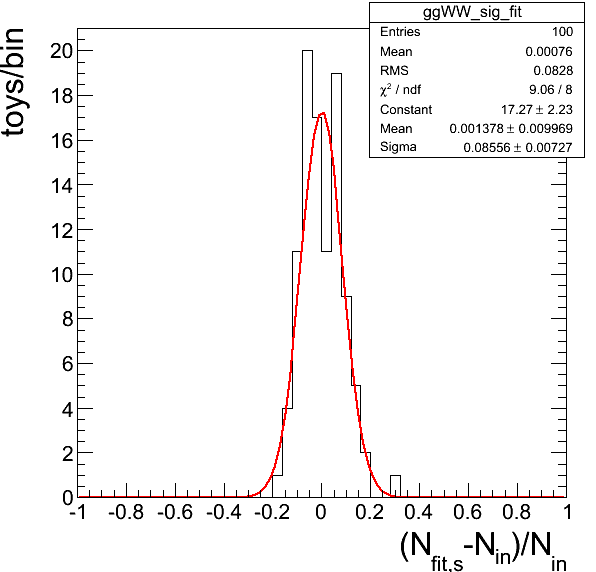
\includegraphics[width=.38\textwidth]{figures/norm_inj125_0j_125_sfit_ggWW.png}
}
\\
\subfigure[Wjets]{
\centering
\label{subfig:norm_inj125_0j_125_sfit_Wjets}
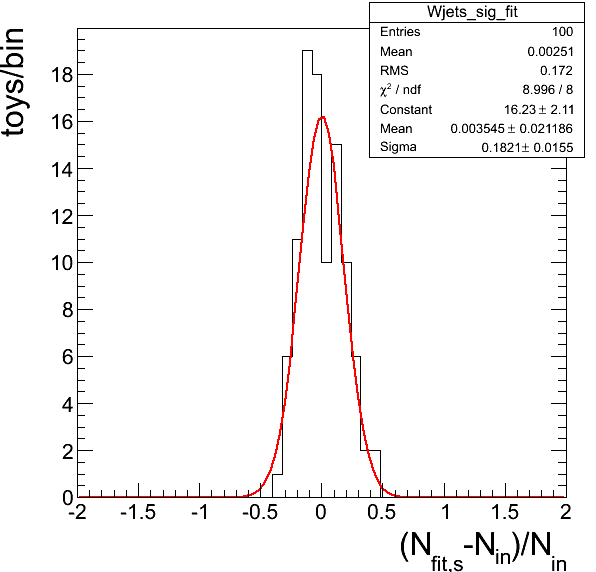
\includegraphics[width=.38\textwidth]{figures/norm_inj125_0j_125_sfit_Wjets.png}
}
\subfigure[Wgamma]{
\centering
\label{subfig:norm_inj125_0j_125_sfit_Wgamma}
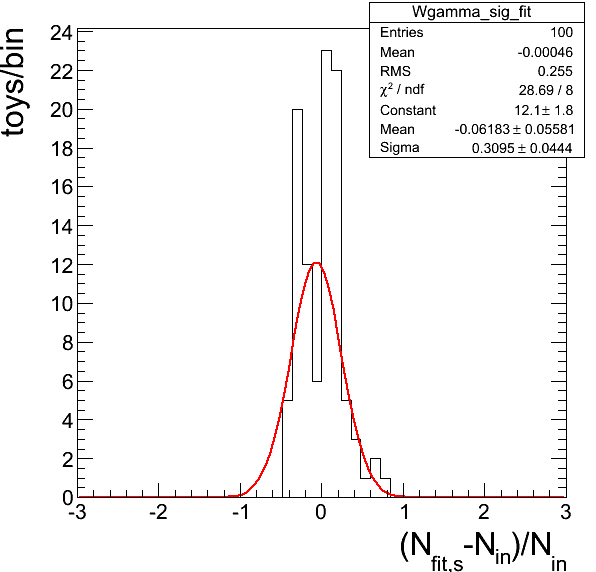
\includegraphics[width=.38\textwidth]{figures/norm_inj125_0j_125_sfit_Wgamma.png}
}
\\
\subfigure[Top]{
\centering
\label{subfig:norm_inj125_0j_125_sfit_Top}
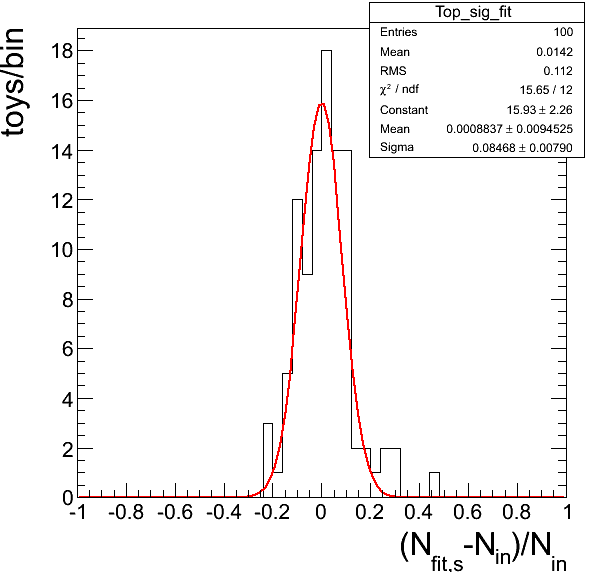
\includegraphics[width=.38\textwidth]{figures/norm_inj125_0j_125_sfit_Top.png}
}
\subfigure[ggH]{
\centering
\label{subfig:norm_inj125_0j_125_sfit_ggH}
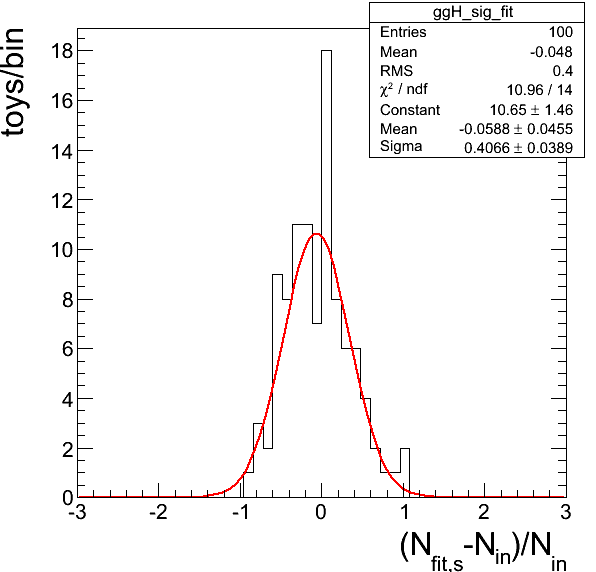
\includegraphics[width=.38\textwidth]{figures/norm_inj125_0j_125_sfit_ggH.png}
}
\caption{Relative shift of post-fit normalization for \mHi=125 \GeV, 0-jet 2D analysis.
A SM Higgs signal with \mHi=125 \GeV\ is injected. Results of background+signal fit are shown.}
\label{fig:norm_inj125_0j_125_sfit}
\end{figure}
%%%%%%%%%%%%%%%%%%%%

%%%%%%%%%%%%%%%%%%%%
\begin{figure}[!hbtp]
\centering
\subfigure[qqWW]{
\centering
\label{subfig:norm_inj125_1j_125_bfit_qqWW}
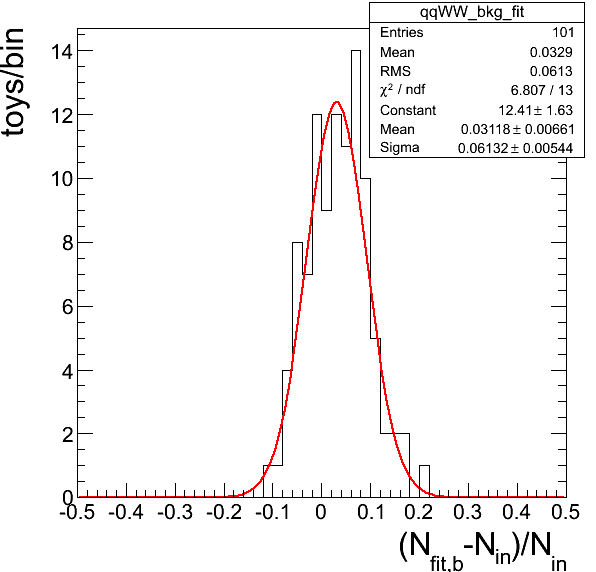
\includegraphics[width=.38\textwidth]{figures/norm_inj125_1j_125_bfit_qqWW.png}
}
\subfigure[ggWW]{
\centering
\label{subfig:norm_inj125_1j_125_bfit_ggWW}
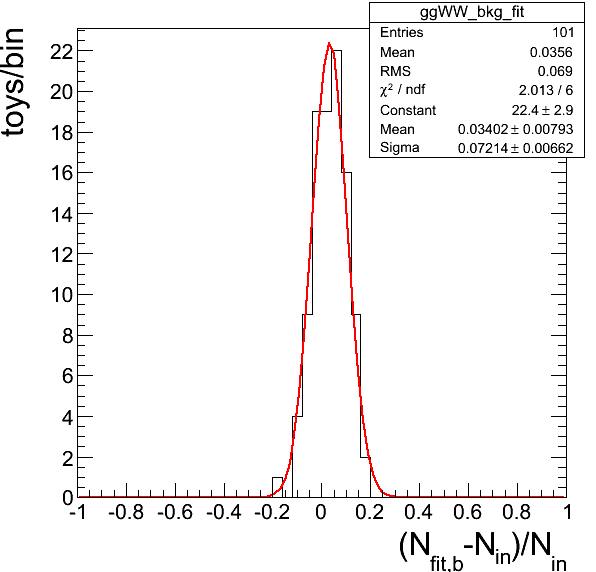
\includegraphics[width=.38\textwidth]{figures/norm_inj125_1j_125_bfit_ggWW.png}
}
\\
\subfigure[Wjets]{
\centering
\label{subfig:norm_inj125_1j_125_bfit_Wjets}
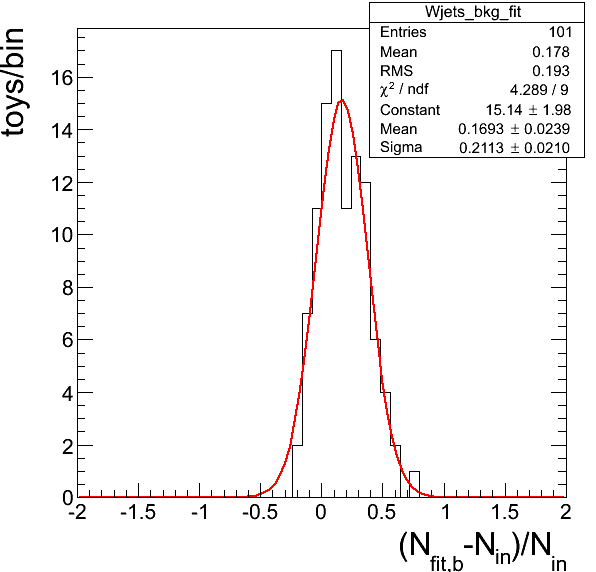
\includegraphics[width=.38\textwidth]{figures/norm_inj125_1j_125_bfit_Wjets.png}
}
\subfigure[Wgamma]{
\centering
\label{subfig:norm_inj125_1j_125_bfit_Wgamma}
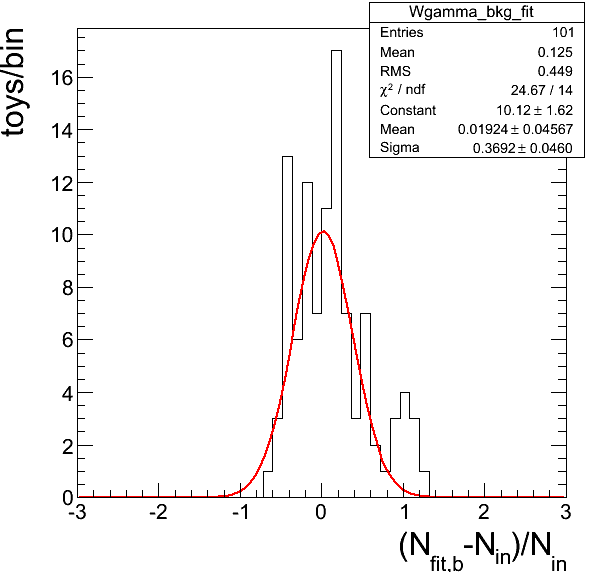
\includegraphics[width=.38\textwidth]{figures/norm_inj125_1j_125_bfit_Wgamma.png}
}
\\
\subfigure[Top]{
\centering
\label{subfig:norm_inj125_1j_125_bfit_Top}
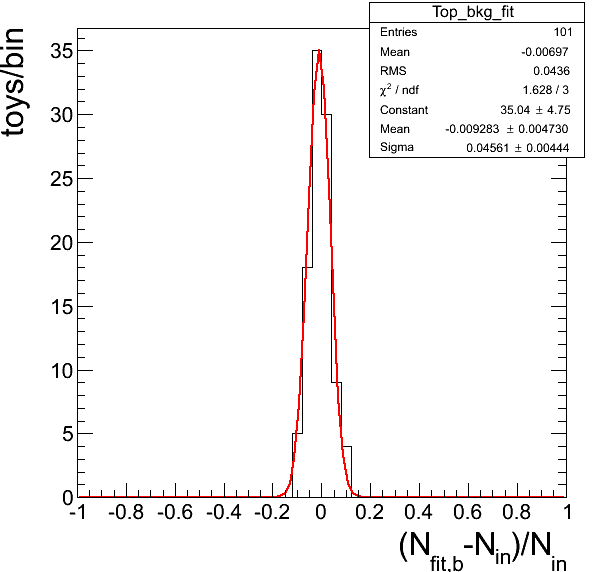
\includegraphics[width=.38\textwidth]{figures/norm_inj125_1j_125_bfit_Top.png}
}
\subfigure[ggH]{
\centering
\label{subfig:norm_inj125_1j_125_bfit_ggH}
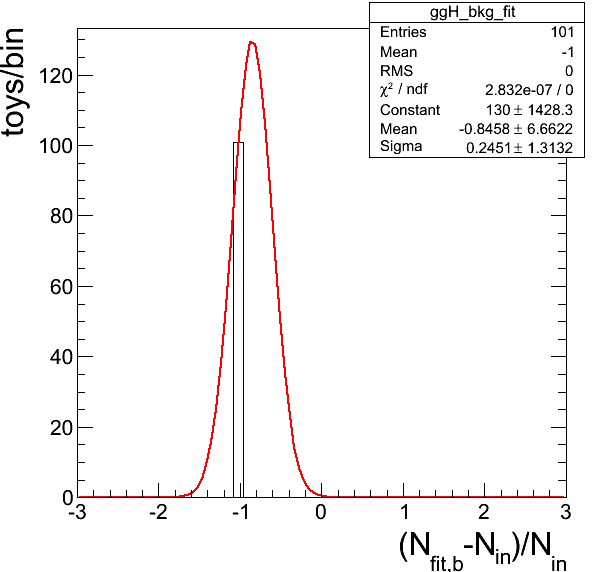
\includegraphics[width=.38\textwidth]{figures/norm_inj125_1j_125_bfit_ggH.png}
}
\caption{Relative shift of post-fit normalization for \mHi=125 \GeV, 1-jet 2D analysis.
A SM Higgs signal with \mHi=125 \GeV\ is injected. Results of background only fit are shown.}
\label{fig:norm_inj125_1j_125_bfit}
\end{figure}
%%%%%%%%%%%%%%%%%%%%

%%%%%%%%%%%%%%%%%%%%
\begin{figure}[!hbtp]
\centering
\subfigure[qqWW]{
\centering
\label{subfig:norm_inj125_1j_125_sfit_qqWW}
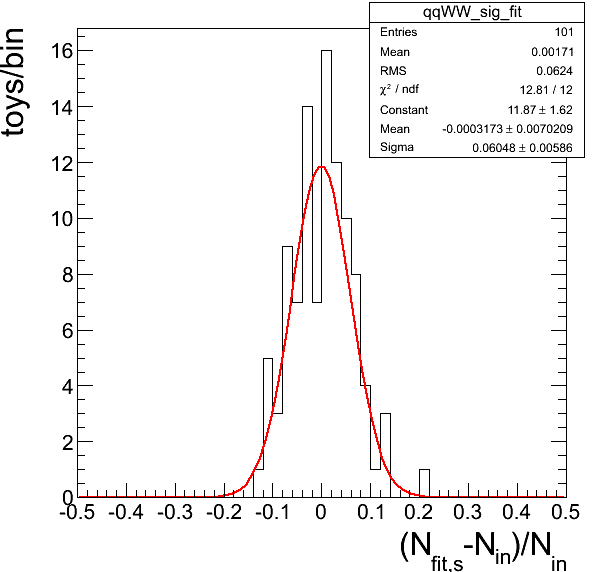
\includegraphics[width=.38\textwidth]{figures/norm_inj125_1j_125_sfit_qqWW.png}
}
\subfigure[ggWW]{
\centering
\label{subfig:norm_inj125_1j_125_sfit_ggWW}
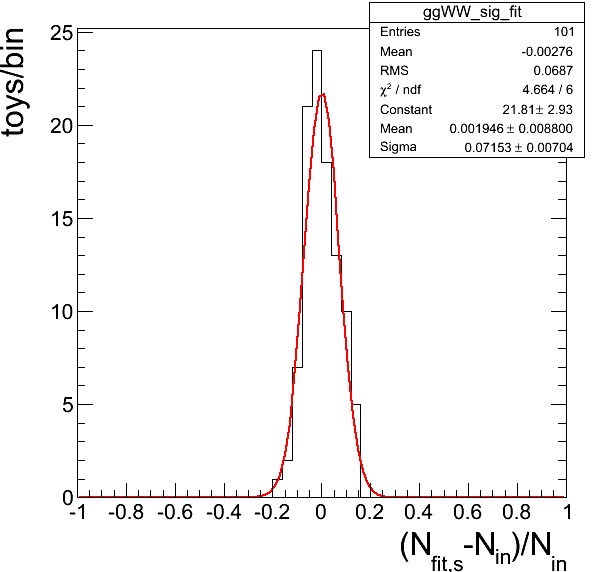
\includegraphics[width=.38\textwidth]{figures/norm_inj125_1j_125_sfit_ggWW.png}
}
\\
\subfigure[Wjets]{
\centering
\label{subfig:norm_inj125_1j_125_sfit_Wjets}
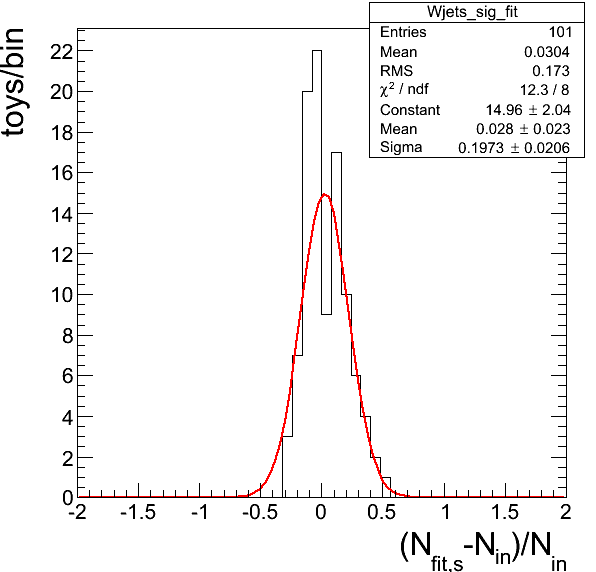
\includegraphics[width=.38\textwidth]{figures/norm_inj125_1j_125_sfit_Wjets.png}
}
\subfigure[Wgamma]{
\centering
\label{subfig:norm_inj125_1j_125_sfit_Wgamma}
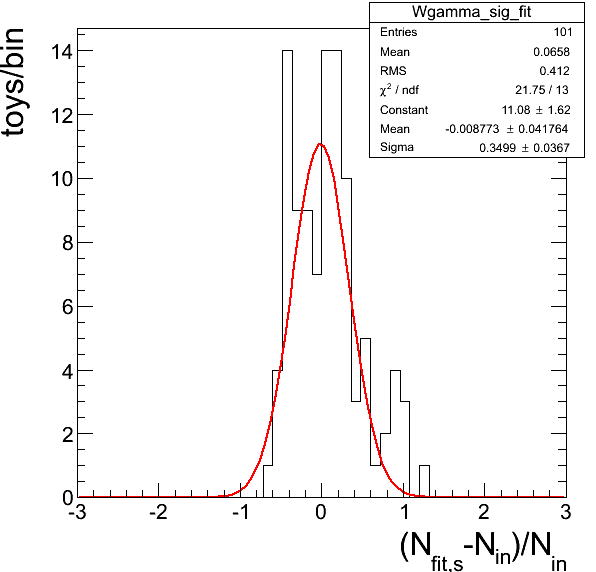
\includegraphics[width=.38\textwidth]{figures/norm_inj125_1j_125_sfit_Wgamma.png}
}
\\
\subfigure[Top]{
\centering
\label{subfig:norm_inj125_1j_125_sfit_Top}
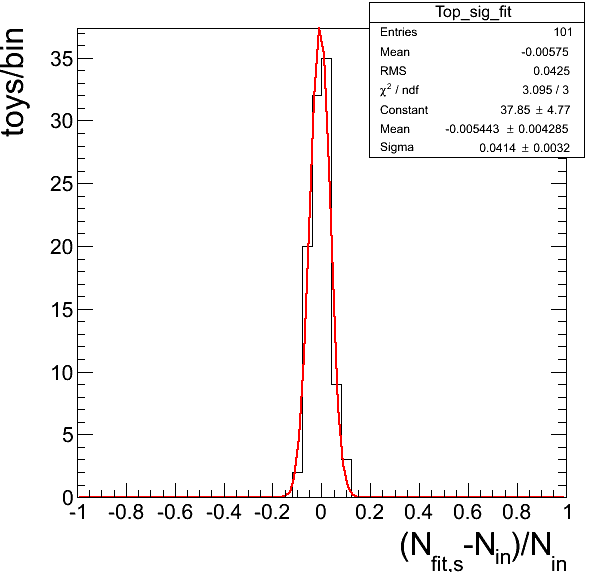
\includegraphics[width=.38\textwidth]{figures/norm_inj125_1j_125_sfit_Top.png}
}
\subfigure[ggH]{
\centering
\label{subfig:norm_inj125_1j_125_sfit_ggH}
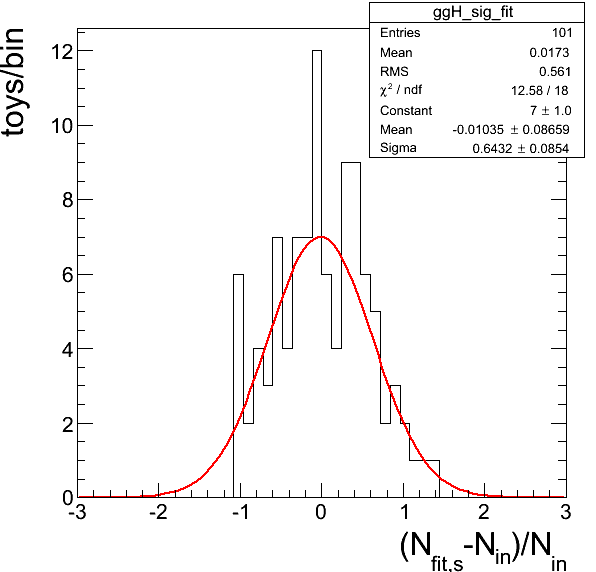
\includegraphics[width=.38\textwidth]{figures/norm_inj125_1j_125_sfit_ggH.png}
}
\caption{Relative shift of post-fit normalization for \mHi=125 \GeV, 1-jet 2D analysis.
A SM Higgs signal with \mHi=125 \GeV\ is injected. Results of background+signal fit are shown.}
\label{fig:norm_inj125_1j_125_sfit}
\end{figure}
%%%%%%%%%%%%%%%%%%%%

\clearpage

%%%%%%%%%%%% MH=200 INJECTION %%%%%%%%%%%%
\subsection{Analysis with \mHi=200 \GeV\ SM Higgs injected}

Post-fit normalization results are summarized in Figures~\ref{fig:norm_inj200_0j_125_bfit}-\ref{fig:norm_inj200_1j_125_sfit}.
B-only and S+B fits are in good agreement and no signal compatible with \mHi=125 \GeV\ is observed; 
signal is absorbed by qqWW and ggWW backgrounds, with biases in the order of 10-50\%.

%%%%%%%%%%%%%%%%%%%%
\begin{figure}[!hbtp]
\centering
\subfigure[qqWW]{
\centering
\label{subfig:norm_inj200_0j_125_bfit_qqWW}
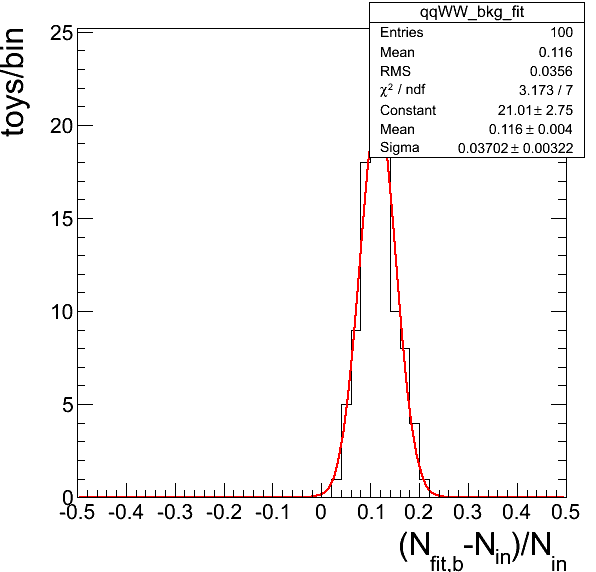
\includegraphics[width=.38\textwidth]{figures/norm_inj200_0j_125_bfit_qqWW.png}
}
\subfigure[ggWW]{
\centering
\label{subfig:norm_inj200_0j_125_bfit_ggWW}
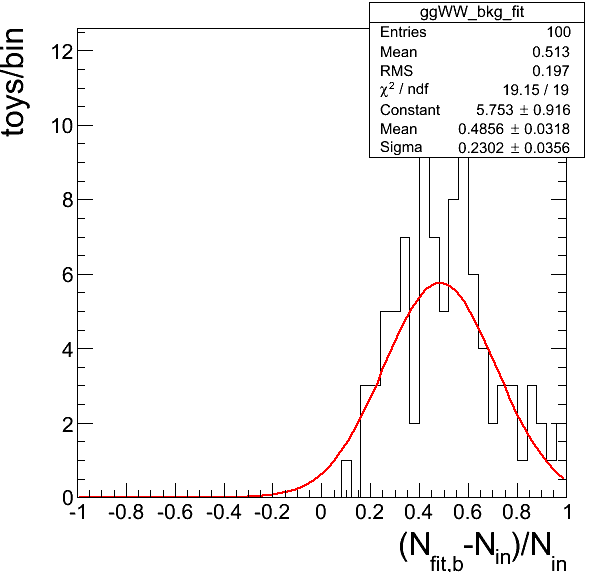
\includegraphics[width=.38\textwidth]{figures/norm_inj200_0j_125_bfit_ggWW.png}
}
\\
\subfigure[Wjets]{
\centering
\label{subfig:norm_inj200_0j_125_bfit_Wjets}
\includegraphics[width=.38\textwidth]{figures/norm_inj200_0j_125_bfit_Wjets.png}
}
\subfigure[Wgamma]{
\centering
\label{subfig:norm_inj200_0j_125_bfit_Wgamma}
\includegraphics[width=.38\textwidth]{figures/norm_inj200_0j_125_bfit_Wgamma.png}
}
\\
\subfigure[Top]{
\centering
\label{subfig:norm_inj200_0j_125_bfit_Top}
\includegraphics[width=.38\textwidth]{figures/norm_inj200_0j_125_bfit_Top.png}
}
\subfigure[ggH]{
\centering
\label{subfig:norm_inj200_0j_125_bfit_ggH}
\includegraphics[width=.38\textwidth]{figures/norm_inj200_0j_125_bfit_ggH.png}
}
\caption{Relative shift of post-fit normalization for \mHi=125 \GeV, 0-jet 2D analysis.
A SM Higgs signal with \mHi=200 \GeV\ is injected. Results of background only fit are shown.}
\label{fig:norm_inj200_0j_125_bfit}
\end{figure}
%%%%%%%%%%%%%%%%%%%%

%%%%%%%%%%%%%%%%%%%%
\begin{figure}[!hbtp]
\centering
\subfigure[qqWW]{
\centering
\label{subfig:norm_inj200_0j_125_sfit_qqWW}
\includegraphics[width=.38\textwidth]{figures/norm_inj200_0j_125_sfit_qqWW.png}
}
\subfigure[ggWW]{
\centering
\label{subfig:norm_inj200_0j_125_sfit_ggWW}
\includegraphics[width=.38\textwidth]{figures/norm_inj200_0j_125_sfit_ggWW.png}
}
\\
\subfigure[Wjets]{
\centering
\label{subfig:norm_inj200_0j_125_sfit_Wjets}
\includegraphics[width=.38\textwidth]{figures/norm_inj200_0j_125_sfit_Wjets.png}
}
\subfigure[Wgamma]{
\centering
\label{subfig:norm_inj200_0j_125_sfit_Wgamma}
\includegraphics[width=.38\textwidth]{figures/norm_inj200_0j_125_sfit_Wgamma.png}
}
\\
\subfigure[Top]{
\centering
\label{subfig:norm_inj200_0j_125_sfit_Top}
\includegraphics[width=.38\textwidth]{figures/norm_inj200_0j_125_sfit_Top.png}
}
\subfigure[ggH]{
\centering
\label{subfig:norm_inj200_0j_125_sfit_ggH}
\includegraphics[width=.38\textwidth]{figures/norm_inj200_0j_125_sfit_ggH.png}
}
\caption{Relative shift of post-fit normalization for \mHi=125 \GeV, 0-jet 2D analysis.
A SM Higgs signal with \mHi=200 \GeV\ is injected. Results of background+signal fit are shown.}
\label{fig:norm_inj200_0j_125_sfit}
\end{figure}
%%%%%%%%%%%%%%%%%%%%

%%%%%%%%%%%%%%%%%%%%
\begin{figure}[!hbtp]
\centering
\subfigure[qqWW]{
\centering
\label{subfig:norm_inj200_1j_125_bfit_qqWW}
\includegraphics[width=.38\textwidth]{figures/norm_inj200_1j_125_bfit_qqWW.png}
}
\subfigure[ggWW]{
\centering
\label{subfig:norm_inj200_1j_125_bfit_ggWW}
\includegraphics[width=.38\textwidth]{figures/norm_inj200_1j_125_bfit_ggWW.png}
}
\\
\subfigure[Wjets]{
\centering
\label{subfig:norm_inj200_1j_125_bfit_Wjets}
\includegraphics[width=.38\textwidth]{figures/norm_inj200_1j_125_bfit_Wjets.png}
}
\subfigure[Wgamma]{
\centering
\label{subfig:norm_inj200_1j_125_bfit_Wgamma}
\includegraphics[width=.38\textwidth]{figures/norm_inj200_1j_125_bfit_Wgamma.png}
}
\\
\subfigure[Top]{
\centering
\label{subfig:norm_inj200_1j_125_bfit_Top}
\includegraphics[width=.38\textwidth]{figures/norm_inj200_1j_125_bfit_Top.png}
}
\subfigure[ggH]{
\centering
\label{subfig:norm_inj200_1j_125_bfit_ggH}
\includegraphics[width=.38\textwidth]{figures/norm_inj200_1j_125_bfit_ggH.png}
}
\caption{Relative shift of post-fit normalization for \mHi=125 \GeV, 1-jet 2D analysis.
A SM Higgs signal with \mHi=200 \GeV\ is injected. Results of background only fit are shown.}
\label{fig:norm_inj200_1j_125_bfit}
\end{figure}
%%%%%%%%%%%%%%%%%%%%

%%%%%%%%%%%%%%%%%%%%
\begin{figure}[!hbtp]
\centering
\subfigure[qqWW]{
\centering
\label{subfig:norm_inj200_1j_125_sfit_qqWW}
\includegraphics[width=.38\textwidth]{figures/norm_inj200_1j_125_sfit_qqWW.png}
}
\subfigure[ggWW]{
\centering
\label{subfig:norm_inj200_1j_125_sfit_ggWW}
\includegraphics[width=.38\textwidth]{figures/norm_inj200_1j_125_sfit_ggWW.png}
}
\\
\subfigure[Wjets]{
\centering
\label{subfig:norm_inj200_1j_125_sfit_Wjets}
\includegraphics[width=.38\textwidth]{figures/norm_inj200_1j_125_sfit_Wjets.png}
}
\subfigure[Wgamma]{
\centering
\label{subfig:norm_inj200_1j_125_sfit_Wgamma}
\includegraphics[width=.38\textwidth]{figures/norm_inj200_1j_125_sfit_Wgamma.png}
}
\\
\subfigure[Top]{
\centering
\label{subfig:norm_inj200_1j_125_sfit_Top}
\includegraphics[width=.38\textwidth]{figures/norm_inj200_1j_125_sfit_Top.png}
}
\subfigure[ggH]{
\centering
\label{subfig:norm_inj200_1j_125_sfit_ggH}
\includegraphics[width=.38\textwidth]{figures/norm_inj200_1j_125_sfit_ggH.png}
}
\caption{Relative shift of post-fit normalization for \mHi=125 \GeV, 1-jet 2D analysis.
A SM Higgs signal with \mHi=200 \GeV\ is injected. Results of background+signal fit are shown.}
\label{fig:norm_inj200_1j_125_sfit}
\end{figure}
%%%%%%%%%%%%%%%%%%%%

\clearpage
